%\documentclass[margin=0mm]{standalone}
%\usepackage{tikz}
%\usepackage{pgfplots}
% \pgfplotsset{compat=newest}
%
%
%\usepgfplotslibrary{groupplots}
%
%\usepackage{currfile,hyperxmp,calc}
%\usetikzlibrary{calc,math}
%\usetikzlibrary{calc,patterns,angles,quotes}
%
%
%\usetikzlibrary{angles,quotes}
%
%\usetikzlibrary{math,matrix,fit,positioning,intersections}
%\usetikzlibrary{patterns,decorations.pathmorphing,decorations.markings}
%\usetikzlibrary{calc}
%\usetikzlibrary{arrows.meta} %needed tikz library
%\usetikzlibrary{quotes,angles}
%
%\usepackage{braket}
%
% 
%
%
%
%
%\begin{document}


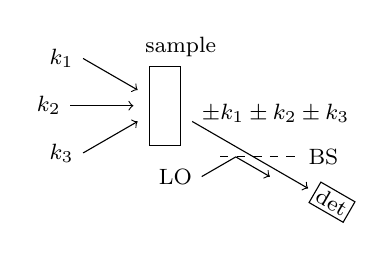
\begin{tikzpicture}[font=\footnotesize]
%\useasboundingbox (0.,0) rectangle (10.6,8.3);

\tikzmath{ \dx1 = -0.4; \dx2=-0.2; \dx3=+0.3;}

\draw (-0.2, -0.5) rectangle (0.2, 0.5) node [above] {sample};


\draw[<-] (0,0) ++ (-150:0.4) -- ++ (-150:0.8)node [left] {$k_3$};
\draw[<-] (0,0) ++ (-180:0.4) -- ++ (-180:0.8) node [left] {$k_2$};
\draw[<-] (0,0) ++ (-210:0.4) -- ++ (-210:0.8) node [left] {$k_1$};

\draw[->] (0,0) ++ (-30:0.4) node[right, yshift=1mm] {$\pm k_1 \pm k_2 \pm k_3$} -- ++ (-30:1.7) node (det) {};

\draw[dashed] (0.7,-0.65) -- ++ (1,0) node[right] {BS};

\draw [->] (0.9, -0.65)  ++ (-150:0.5) node [left ,align=right] {LO} -- (0.9, -0.65)  -- ++(-30:0.5);

\begin{scope}[shift= (det), rotate=-30]
\draw (0.1, -0.15) rectangle node[rotate=-30] {det} (0.6, 0.15) ;
\end{scope}

\end{tikzpicture}



%\end{document}